\documentclass[t]{beamer}
\usepackage[utf8]{inputenc} % to be able to type unicode text directly
%\usepackage{inconsolata} % for a nicer (e.g. non-courier) tt family font

\usepackage{graphicx} % to include figures
\usepackage{animate} % to include figures
%\usepackage{hyperref,url} % to make clickable hyperlinks
%\usepackage{minted} % for code insets
%\usepackage{array} % to fine-tune tabular spacing
%\usepackage{graphbox} % to fine-tune image alignment
%\usepackage{bbm} % for blackboard 1
\usepackage{soul} % for colored strikethrough

\colorlet{darkgreen}{black!50!green} % used for page numbers
\definecolor{term}{rgb}{.9,.9,.9} % used for code insets
\colorlet{darkred}{black!50!red}
\colorlet{lightgray}{black!50!gray}

\newcommand{\reference}[1] {{\scriptsize \color{gray}  #1 }}
\newcommand{\referencep}[1] {{\tiny \color{gray}  #1 }}
\newcommand{\unit}[1] {{\tiny \color{gray}  #1 }}

% coco's macros
\def\R{\mathbf{R}}
\def\F{\mathcal{F}}
\def\x{\mathbf{x}}
\def\u{\mathbf{u}}

%% disable spacing around verbatim
%\usepackage{etoolbox}
%\makeatletter
%\preto{\@verbatim}{\topsep=0pt \partopsep=0pt }
%\makeatother

% disable headings, set slide numbers in green
\mode<presentation>
\setbeamercolor*{author in head/foot}{parent=none}
\setbeamercolor*{title in head/foot}{parent=none}
\setbeamercolor*{date in head/foot}{parent=none}
\defbeamertemplate*{footline}{infoline theme}
{
  \leavevmode%
  \hfill\color{darkgreen}
   \insertframenumber{} / \inserttotalframenumber\hspace*{2ex}
  \vskip0pt%
}

% select red color for strikethrough
\makeatletter
\newcommand\SoulColor{%
  \let\set@color\beamerorig@set@color
  \let\reset@color\beamerorig@reset@color}
\makeatother
\newcommand<>{\St}[1]{\only#2{\SoulColor\st{#1}}}
\setstcolor{red}

\mode<all>
\setbeamertemplate{navigation symbols}{}



\begin{document}

\begin{frame}
A Gaussian volcano:
\[
	u(x,y)
	=
	200
	\left( 1+\tfrac13 x \right)
	\left(
		\tfrac{13}{10}e^{-10\left(x^2+y^2\right)}
		-e^{-20\left(x^2+y^2\right)}
	\right)
\]

Direct shading model~{\color{gray}[1]}:
\[
	I(x,y) = \left({
		{\color{red}\alpha}u_x
		+
		{\color{red}\beta}u_y
		+
		{\color{red}\gamma}
}\right)/{\sqrt{u_x^2+u_y^2+1}}
\]

\vfill

\begin{tabular}{cc}
	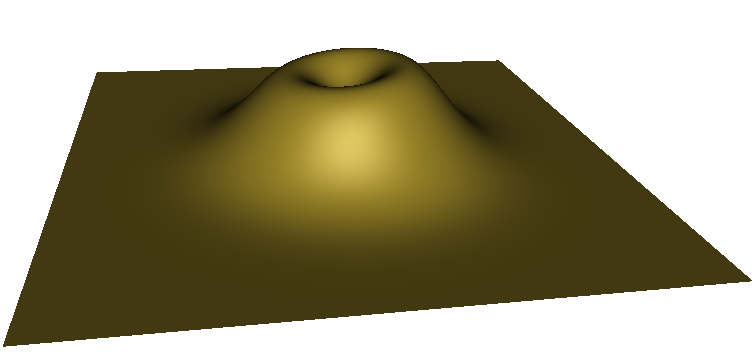
\includegraphics[width=0.5\linewidth]{f/volcano3d.png} &
	%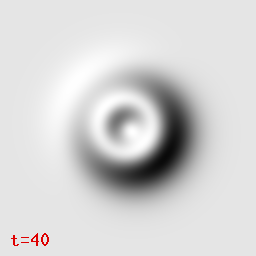
\includegraphics[width=0.25\linewidth]{f/cview_4.png} \\
	\animategraphics[width=0.25\linewidth,loop,autoplay]{4}{f/cview_}{1}{36} \\
	$z=u(x,y)$ &
	$I(x,y)$ \\
	&
	\tiny
	$({\color{red}\alpha},{\color{red}\beta})
	=
	(\cos{\color{red}t},\sin{\color{red}t})$
\end{tabular}

\vfill

\referencep{
	[1] Horn-Brooks,
	\emph{The variational approach to shape form shading},
	1986
}

\end{frame}



\end{document}


% vim:sw=4 ts=4 spell spelllang=en:
